\documentclass[12pt,letterpaper]{article}
\usepackage[utf8]{inputenc}
\usepackage[left=2cm,right=2cm,top=2cm,bottom=2cm]{geometry}
\usepackage{multirow}
\title{Informe Oracle}
\author{Juan Rodriguez}
\date{November 2018}

\usepackage{natbib}
\usepackage{graphicx}

\begin{document}
    
    \begin{center}
        
\includegraphics[width=4cm]{Imagenes/upt-logo.png}\\
        \vspace{12pt}
        \vspace{12pt}
        \large\textbf{UNIVERSIDAD PRIVADA DE TACNA}\\
        \vspace{12pt}
        \vspace{12pt}
        \large{FACULTAD DE INGENIERIA}\\
        \vspace{12pt}
        \vspace{12pt}
        \large{Escuela Profesional de Ingeniería de Sistemas}\\
        \vspace{12pt}
        \vspace{12pt}
        \textbf{INSTALACION DE ORACLE DATABASE}\\
        \vspace{12pt}
        \vspace{12pt}
        Curso: Bases de Datos II\\
        \vspace{12pt}
        Docente: Ing. Patrick Cuadros\\
        \vspace*{12pt}
           \begin{flushleft}
        Alumno:\\
        \vspace{12pt}
        Rodriguez Mamani, Juan Rigoberto\hfill (2017057862)\\

        \end{flushleft}
        \vspace{100pt}

        Tacna – Perú\\
            2018
        \vspace{12pt}
        
    \end{center}
    \thispagestyle{empty} % CARATULA SIN NUMERO
    \newpage
    \tableofcontents % INDICE
    \thispagestyle{empty} % INDICE SIN NUMERO
    \newpage
    \setcounter{page}{1} % REINICIAR CONTADOR DE PAGINAS DESPUES DEL INDICE

    \section{INTRODUCCION}
\begin{enumerate}
\vspace{12pt}

Oracle es básicamente un herramienta cliente/servidor para la gestión de base de datos, es un producto vendido a nivel mundial, aunque la gran potencia que tiene y su elevado precio hace que solo se vea en empresas muy grandes y multinacionales, por norma general.\\

En el desarrollo de paginas Web pasa lo mismo como es un sistema muy caro no está tan extendido como otras bases de datos, por ejemplo, Access, MySQL, SQL Server etc.\\


Oracle como antes lo mencionamos se basa en la tecnología cliente/ servidor, pues bien, para su utilización primero seria necesario la instalación de la herramienta servidor ( Oracle8i ) y posteriormente podríamos atacar a la base de datos desde otros equipos con herramientas de desarrollo como Oracle Designer y Oracle Developer, que son las herramientas de programación sobre Oracle a partir de esta premisa vamos a desarrollar las principales acepciones de Oracle y sus aplicaciones en las distintas ares de trabajo.\\

Es posible lógicamente atacar a la base de datos a través del SQL plus incorporado en el paquete de programas Oracle para poder realizar consultas, utilizando el lenguaje SQL.\\

El Developer es una herramienta que nos permite crear formularios en local, es decir, mediante esta herramienta nosotros podemos crear formularios, compilarlos y ejecutarlos, pero si queremos que los otros trabajen sobre este formulario deberemos copiarlo regularmente en una carpeta compartida para todos, de modo que, cuando quieran realizar un cambio, deberán copiarlo de dicha carpeta y luego volverlo a subir a la carpeta.\\

Este sistema como podemos observar es bastante engorroso y poco fiable pues es bastante normal que las versiones se pierdan y se machaquen con frecuencia. La principal ventaja de esta herramienta es que es bastante intuitiva y dispone de un modo que nos permite componer el formulario, tal y como lo haríamos en Visual Basic o en Visual C, esto es muy de agradecer.\\

\end{enumerate}

    \section{OBJETIVOS}
\begin{enumerate}
\vspace{12pt}
-Poner en practica los conocimientos necesarios para realizar la Instalación de un servidor de Base de Datos Oracle sobre un sistema operativo Linux.\\

-Realizar de forma correcta la instalación de la Base de Datos Oracle dentro de un ambiente virtualizado.\\


\end{enumerate}

    \section{MARCO TEORICO}
\begin{enumerate}
\vspace{12pt}
\begin{center}

\includegraphics[width=10cm]{Imagenes/Oracle_logo.png}\\
\end{center}

\subsection{Definición}
Oracle Database es un sistema de gestión de base de datos de tipo objeto-relacional (ORDBMS, por el acrónimo en inglés de Object-Relational Data Base Management System), desarrollado por Oracle Corporation.\\
Su dominio en el mercado de servidores empresariales había sido casi total hasta que recientemente tiene la competencia del Microsoft SQL Server y de la oferta de otros RDBMS con licencia libre como PostgreSQL, MySQL o Firebird.\\
Las últimas versiones de Oracle han sido certificadas para poder trabajar bajo GNU/Linux.\\


\subsection{Historia}
Oracle surge en 1977 bajo el nombre de SDL (Software Development Laboratories).
En 1979, SDL cambia su nombre por Relational Software, Inc. (RSI).
La fundación de SDL fue motivada principalmente a partir de un estudio sobre los SGBD (Sistemas Gestores de Base de Datos) de George Koch. Computer World definió este estudio como uno de los más completos jamás escritos sobre bases de datos. Este artículo incluía una comparativa de productos que dirigía a Relational Software como el más completo desde el punto de vista técnico. 

La tecnología Oracle se encuentra prácticamente en todas las industrias alrededor del mundo y en las oficinas de 98 de las 100 empresas Fortune 100. Oracle es la primera compañía de software que desarrolla e implementa software para empresas cien por ciento activado por Internet a través de toda su línea de productos: base de datos, aplicaciones comerciales y herramientas de desarrollo de aplicaciones y soporte de decisiones. Oracle es el proveedor mundial líder de software para administración de información, y la segunda empresa de software.\\

\textbf {Oracle, a partir de la versión 10g Release 2, cuenta con 7 ediciones:}\\
Enterprise Edition (EE).\\
Standard Edition (SE).\\
Standard Edition One (SE1).\\
Standard Edition 2 (SE2).\\
Express Edition (XE).\\
Personal Edition (PE).\\
Lite Edition (LE).\\
\vspace{12pt}\\

\end{enumerate}
    \section{REQUERIMIENTOS}
\begin{enumerate}
\vspace{12pt}\\

\subsection{Conocimientos}
Para el desarrollo de esta práctica se requerirá de los siguientes conocimientos básicos:\\
- Conocimientos básicos de comandos Linux a nivel de consola o terminal de texto.\\
- Conocimientos básicos de redes locales.\\

\vspace{12pt}\\
\subsection{Hardware}
Se necesitará un PC (computadora personal), con las siguientes características:\\
- 01 procesador de doble núcleo o superior.\\
- 4Gb de memoria física (RAM) o superior.\\
- Disco duro con 100Gb de capacidad y al menos 30Gb de espacio libre.\\
- Unidad Lector de DVD.\\
- Interfaz de Red Ethernet activa.\\

\vspace{12pt}\\
\subsection{Software}
Asimismo se necesita los siguientes aplicativos:\\
- Sistema Operativo Windows XP o superior preinstalado, de preferencia actualizado con todos los parches de seguridad.\\
- Instalador de Oracle Linux Release 5 (En DVD o archivo de tipo imagen .ISO).\\
- Instalador de Oracle Database 11g R2 (En DVD o archivo de tipo imagen .ISO).\\
- Instalador de Virtualbox versión 4.x o superior.\\


\end{enumerate}

    \section{DESARROLLO}
\begin{enumerate}

\vspace{12pt}
\subsection{PARTE I: Instalación Hyper-V}

\textbf {1. Verificar Edición de Windows 10:} El Hyper V es una característica de Windows 10 en las versiones PRO y Educational, para esto primero verificaremos si nuestro sistema pertenece a alguna de esas ediciones.
\begin{center}
  
\includegraphics[width=15cm]{Imagenes/Windows_Education.png}
\end{center}
\vspace{15pt}\\

\textbf {2. Buscar la opción de Características de Windows:} Nos dirigimos al Menu del Windows 10 y buscamos la opción de "Activar o desactivar las caracterísitcas de Windows".\\
\begin{center}
  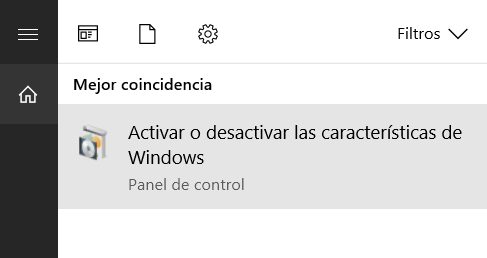
\includegraphics[width=15cm]{Imagenes/Activar_Caracteristicas.png}
\end{center}
\break

\textbf {3. Activar Característica Hyper-V:} Buscamos la opción llamada "Hyper V" y lo activamos.\\
\begin{center}
  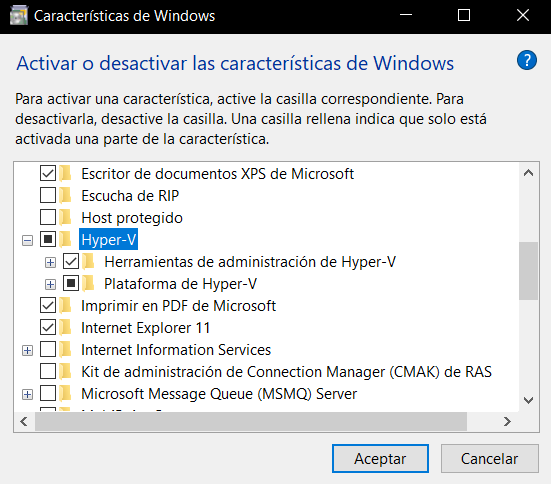
\includegraphics[width=11cm]{Imagenes/Activar_Hyper_V.png}
\end{center}
\vspace{12pt}\\

\textbf {4. Reiniciar el Sistema Operativo:} Con la finalidad de que se apliquen los cambios, es necesario reiniciar el equipo.
\begin{center}
  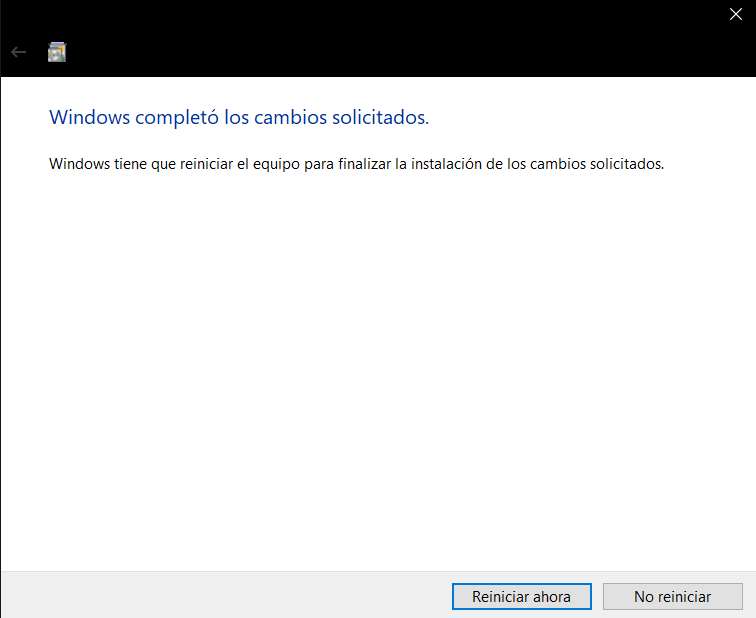
\includegraphics[width=11cm]{Imagenes/Reiniciar.png}
\end{center}
\break

\textbf {5. Hyper V correctamente habilitado:} Una vez reiniciada la computadora, ya podremos abrir nuestro Hyper-V que estará listo para ser configurada.\\
\begin{center}
  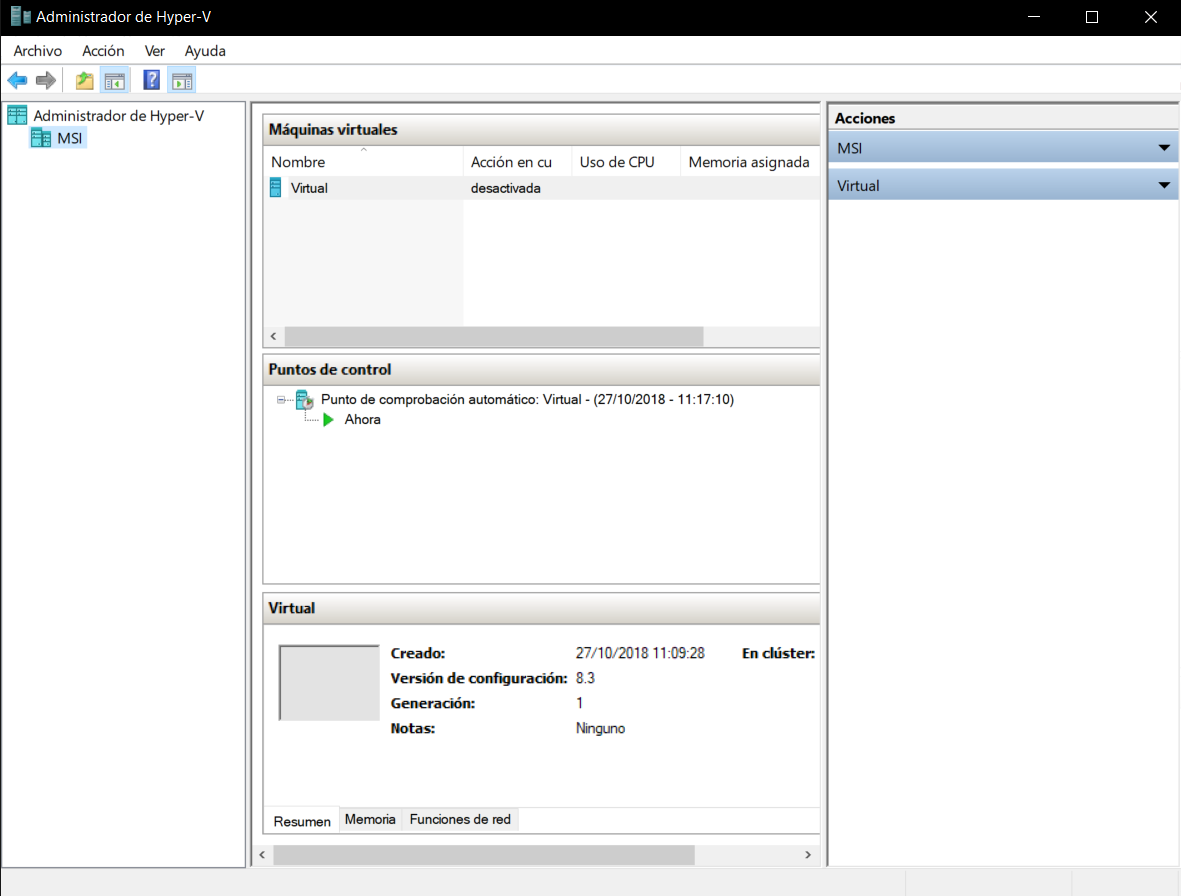
\includegraphics[width=14cm]{Imagenes/Hyper_V.png}
\end{center}
\break

\subsection{PARTE II: Configuración Hyper-V}

\textbf {1. Configurar el Hyper-V:} Una vez habilitado nuestro Hyper V, debemos configurarlo, para eso nos dirigimos a "Acciones - Configuración de Hyper-V
\begin{center}
  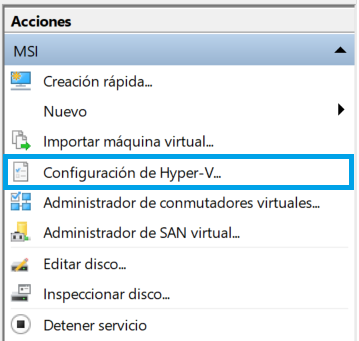
\includegraphics[width=9cm]{Imagenes/Acciones_Configuracion.png}
\end{center}
\vspace{12pt}\\

\textbf {2. Configurar la ruta de los Discos duros:} Ahora pasaremos a asignarles una ruta donde se almacenará nuestros Discos duros, en este caso la ruta será la que se muestra en la imagen.
\begin{center}
  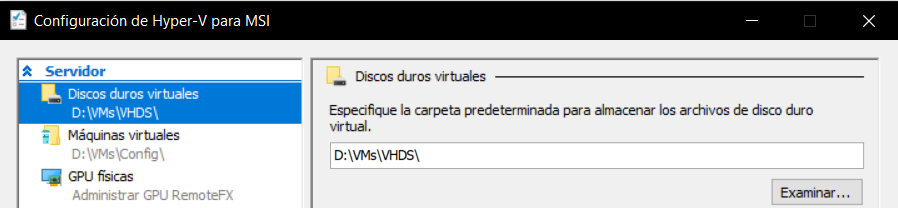
\includegraphics[width=14cm]{Imagenes/Configuracion_Discos.png}
\end{center}
\vspace{12pt}\\


\textbf {3. Configurar la ruta de las Máquinas virtuales:} Del mismo modo pasaremos a configurar la ruta de dónde se guardarán nuestras máquinas virtuales.
\begin{center}
  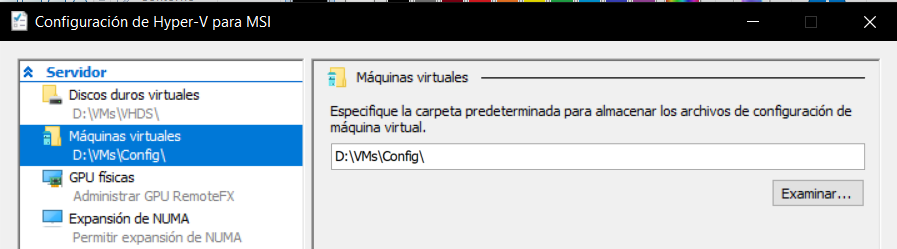
\includegraphics[width=14cm]{Imagenes/Configuracion_Maquinas.png}
\end{center}
\vspace{12pt}\\

\textbf {4. Crear una nueva máquina virtual:} Una vez configurado nuestro Hyper-V crearemos una nueva máquina para eso nos dirigiremos a "Acciones - Nuevo - Maquina Virtual."
\begin{center}
  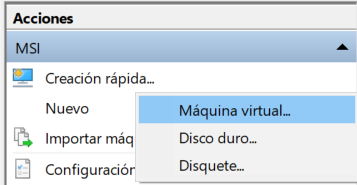
\includegraphics[width=11cm]{Imagenes/Nueva_Maquina.png}
\end{center}
\vspace{15pt}\\

\textbf {5. Asignar Nombre y la ubicación:} En esta parte de la creación, le colocaremos el nombre de "OEL 6.6" ya que instalaremos una versión de Oracle Data Base.
\begin{center}
  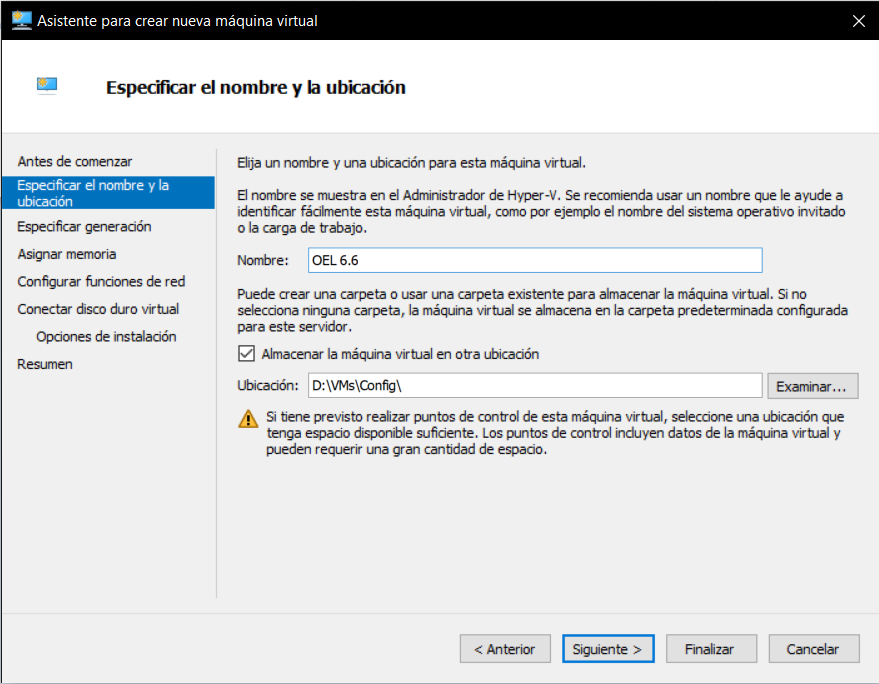
\includegraphics[width=13cm]{Imagenes/Especificar_Nombre.png}
\end{center}
\break

\textbf {6. Especificar Generación:} Eligiremos la Generación por defecto. 
\begin{center}
  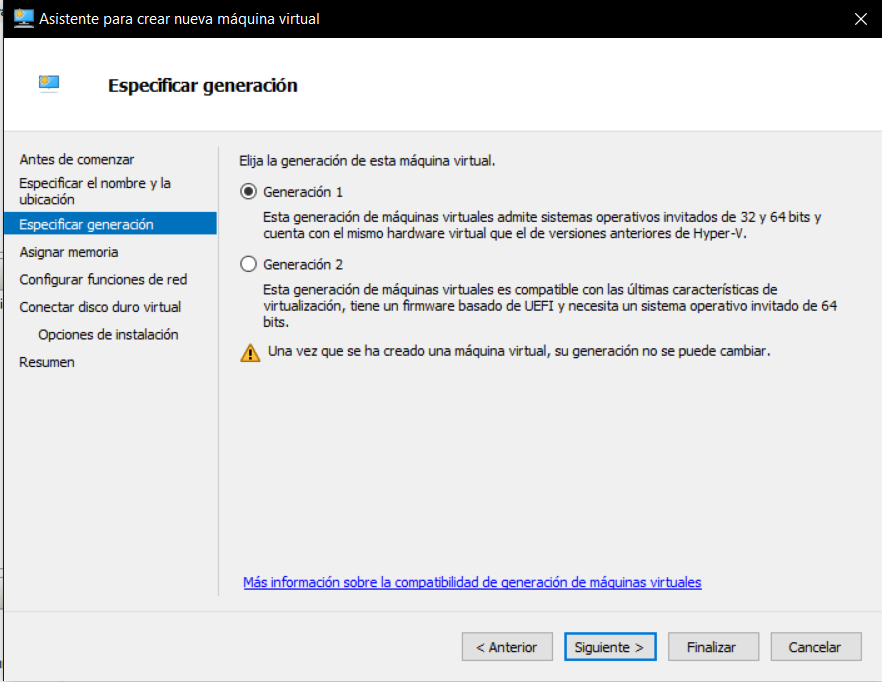
\includegraphics[width=13cm]{Imagenes/Especificar_Generacion.png}
\end{center}
\vspace{12pt}\\

\textbf {7. Asignar Memoria:} Asignaremos un total de 2048 MB de memoria RAM, con la finalidad de que la performance sea mas óptima.
\begin{center}
  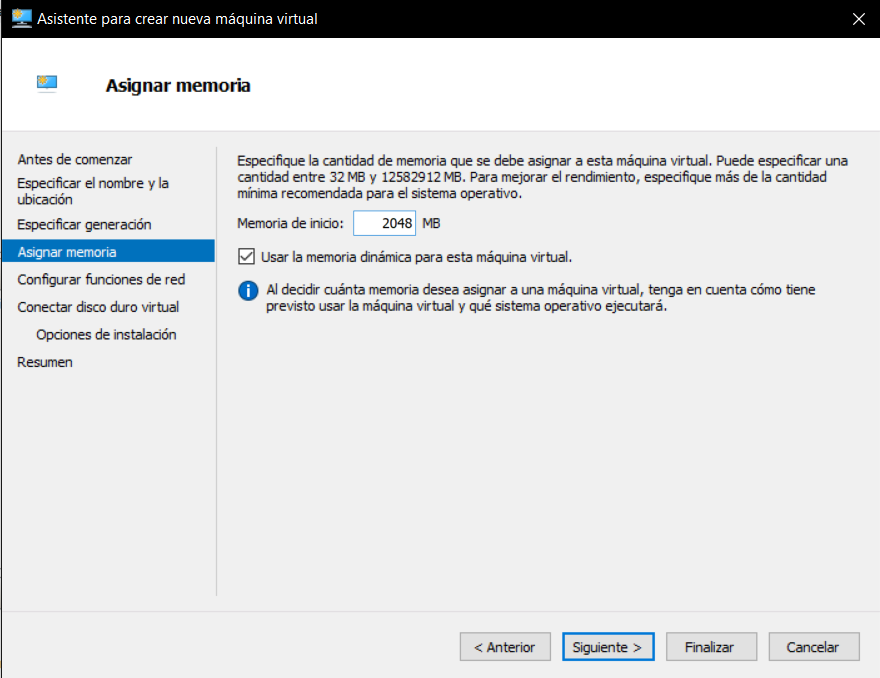
\includegraphics[width=13cm]{Imagenes/Asignar_Memoria.png}
\end{center}
\break

\textbf {8. Conectar Disco Duro:} Si asi lo queremos, especificaremos la ruta de nuestro disco duro.
\begin{center}
  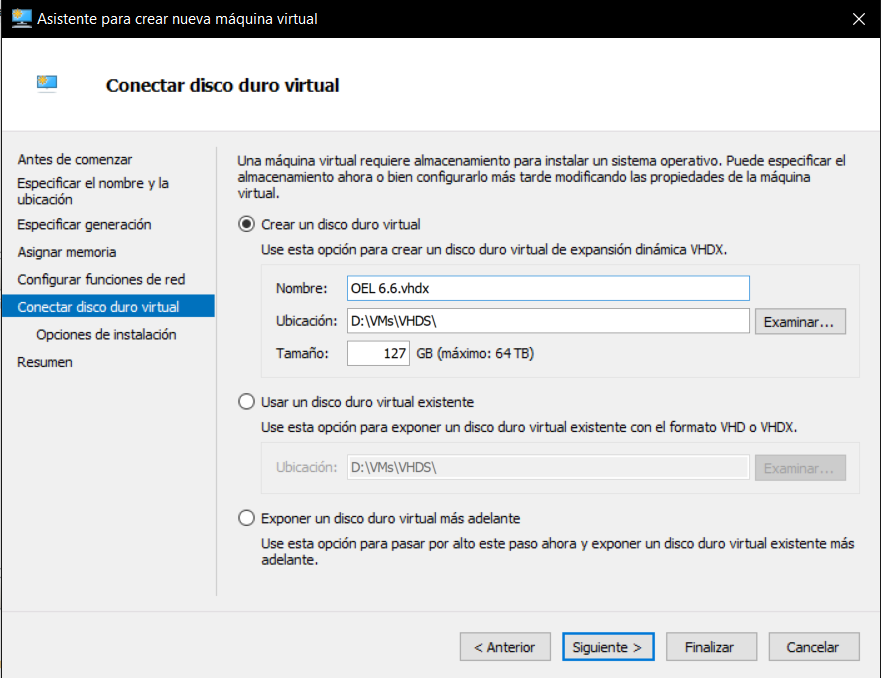
\includegraphics[width=13cm]{Imagenes/Conectar_Disco.png}
\end{center}
\vspace{12pt}\\

\textbf {9. Opciones de instalación:} También podemos espeficiar la ruta de nuestro instaladoro podemos optar de configurarlo mas adelante.
\begin{center}
  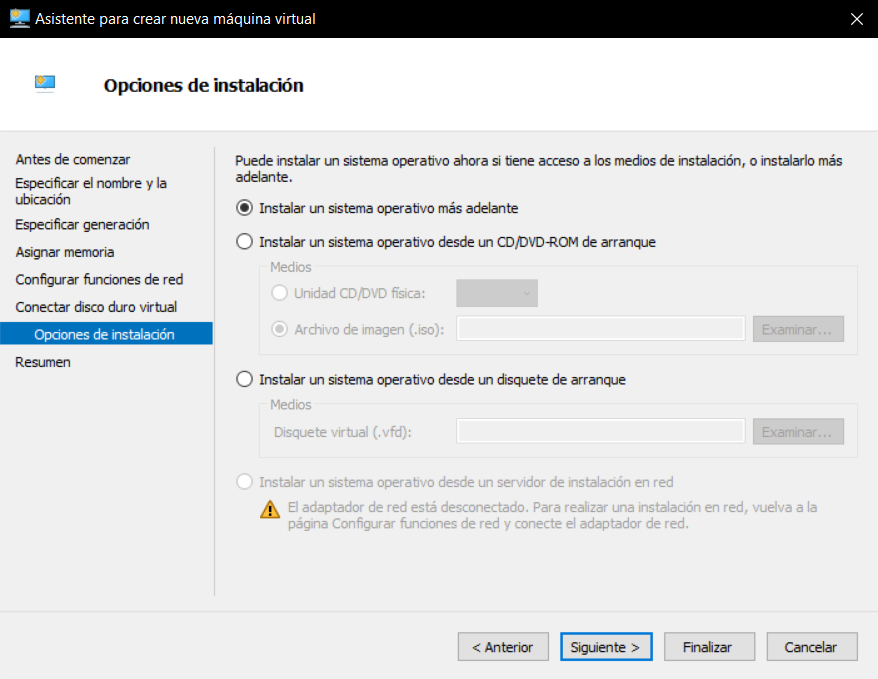
\includegraphics[width=13cm]{Imagenes/Opciones_Instalacion.png}
\end{center}
\break

\textbf {10. Resumen:} Como último paso verificaremos el resumen de nuestra instalación, si todo esta conforme lo hemos configurado, pasaremos dar clic en “Finalizar” para que así comience nuestra instalación.
\begin{center}
  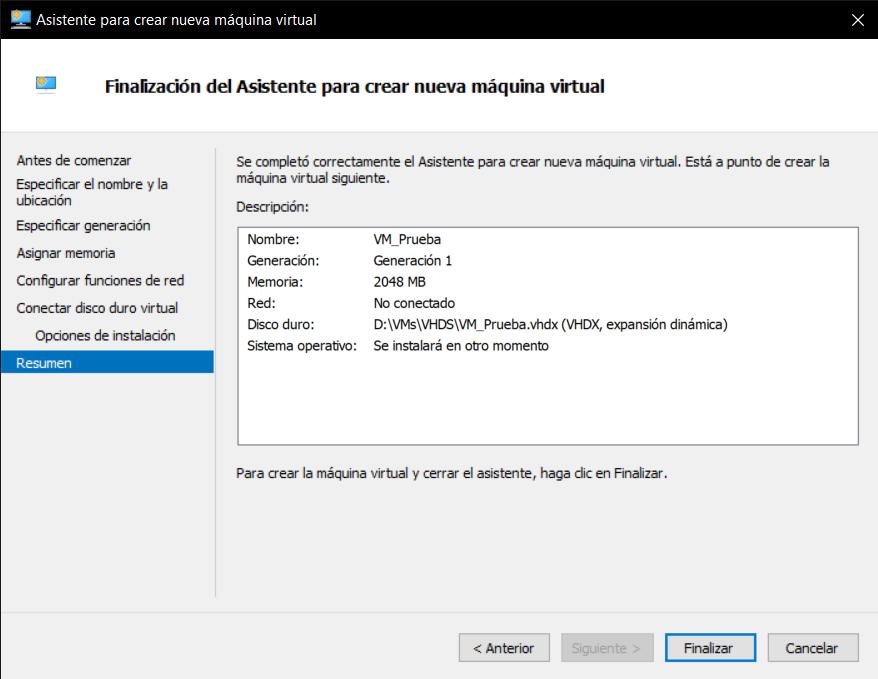
\includegraphics[width=13cm]{Imagenes/Resumen.png}
\end{center}
\break

\subsection{PARTE III: Instalación de Oracle Database Server}
\vspace{12pt}\\

\textbf {Paso 1.-} En el sistema operativo Oracle Linux Server, iniciar sesión con el usuario root. Para lo cual introducir el nombre del usuario y su respectiva contraseña en la pantalla de inicio de sesión.
\vspace{12pt}\\

\textbf {Paso 2.-} Una vez iniciada la sesión montar la unidad de DVD o archivo imagen conteniendo el aplicativo de instalación de Oracle Linux Server, para esto salir o escapar de la máquina y utilizar el menú Devices (Dispositivos) de la ventana de la máquina virtual para activar o montar la unidad de DVD o Archivo de Imagen en la máquina virtual, como se muestra en la siguiente imagen.
\begin{center}
  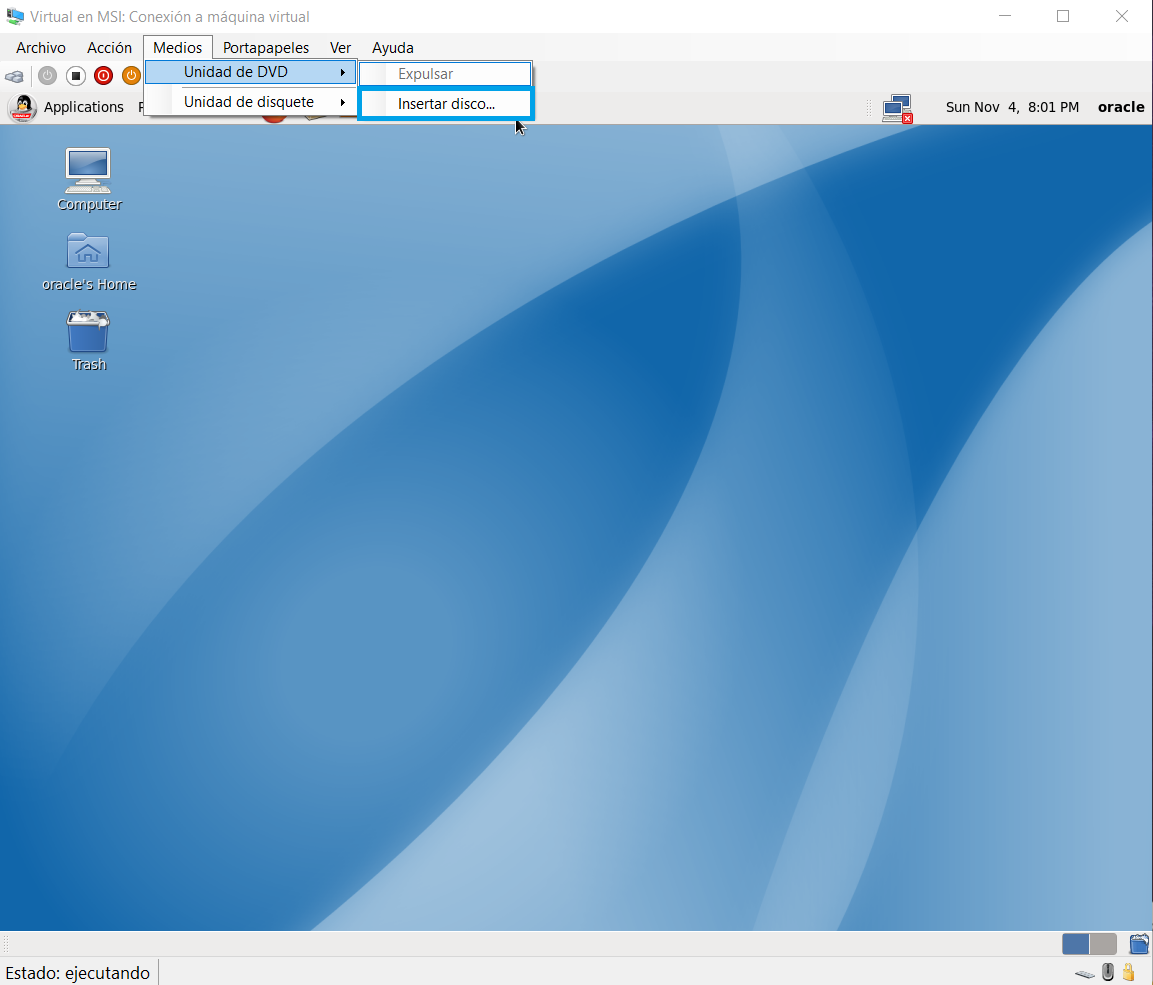
\includegraphics[width=12cm]{Imagenes/Oracle_Database/2_Insertar_Disco.png}
\end{center}
\break

\textbf {Paso 3.-} - Una vez montada la unidad de DVD o archivo de tipo imagen en la maquina virtual, se abrirá una carpeta mostrando el contenido, tomar en cuenta el nombre de la carpeta que será utilizado posteriormente.
\vspace{12pt}\\

\textbf {Paso 4.-} Aperturar una ventana de Terminal, para esto abrir el menú Applications (Aplicaciones), y dentro del submenú Accessories (Accesorios), seleccionar la opción Terminal.
\begin{center}
  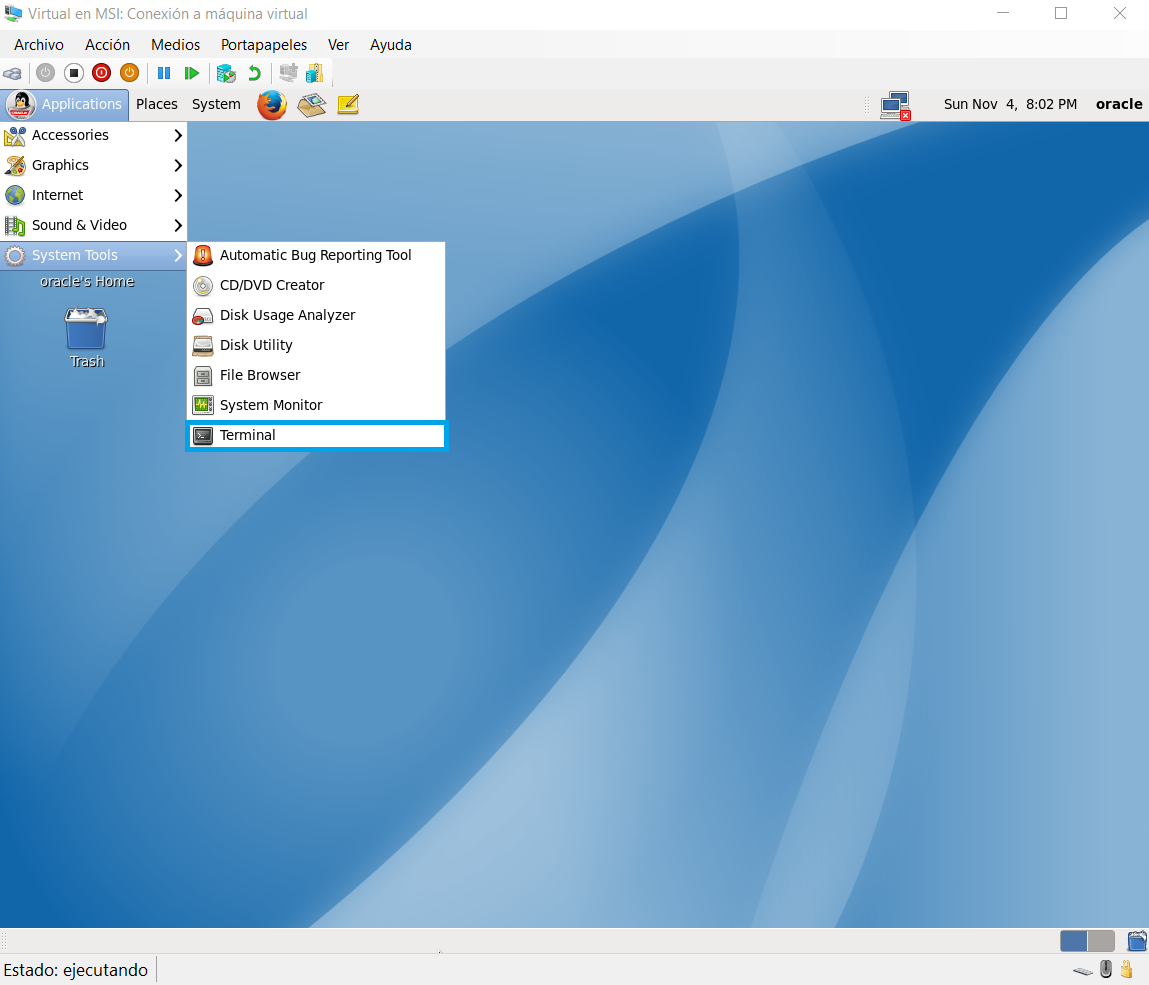
\includegraphics[width=11cm]{Imagenes/Oracle_Database/4_Abrir_Terminal.png}
\end{center}
\vspace{12pt}\\

\textbf {Paso 5.-} Dentro de la ventana de Terminal, acceder a la carpeta de CD/DVD anteriormente montada (para la presente instalación la carpeta tiene el nombre “OL6.6 i386 dvd 20110728” aunque este nombre puede variar). Utilizar el siguiente comando:

\begin{center}
  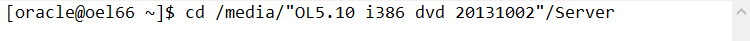
\includegraphics[width=15cm]{Imagenes/Oracle_Database/Paso_5.png}
\end{center}
\break

\textbf {Paso 6.-} Seguidamente se deberán instalar algunos paquetes pre requisitos para la instalación de Oracle Database Server. Para lo cual se deberá ejecutar el siguiente comando desde el Terminal:

\begin{center}
  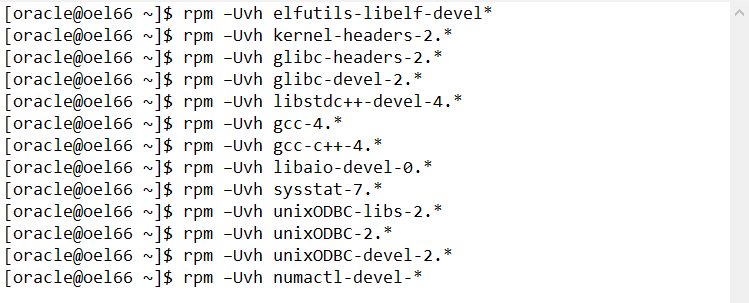
\includegraphics[width=12cm]{Imagenes/Oracle_Database/Paso_6.png}
\end{center}
\vspace{12pt}\\

\textbf {Paso 7.-} Asimismo para la instalación de Oracle Database, se deberá crear dos grupos de usuarios “oinstall” y “dba”, así como una cuenta de usuario llamada “oracle” que pertenecerá a ambos grupos, finalmente de deberá asignar una contraseña al usuario “oracle” la cual para esta instalación también será “oracle”. Utilizar los siguiente comandos para realizar este paso.

\begin{center}
  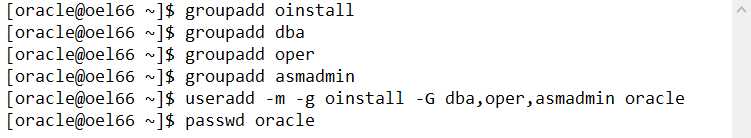
\includegraphics[width=12cm]{Imagenes/Oracle_Database/Paso_7.png}
\end{center}
\vspace{12pt}\\

\textbf {Paso 8.-} Ahora es necesario crear la ruta o la carpeta en donde se instalará Oracle Database, así como establecer los permisos necesarios para que el usuario “oracle” puede accesar y modificar esta carpeta, para lo cual será necesario ejecutar los siguiente comandos.

\begin{center}
  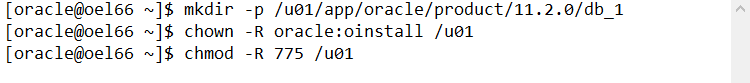
\includegraphics[width=12cm]{Imagenes/Oracle_Database/Paso_8.png}
\end{center}
\vspace{12pt}\\

\textbf {Paso 9.-} A continuación se necesitará configurar algunos parámetros del kernel, para eso será necesario editar el archivo /etc/sysctl.conf, puede utilizar el editor de su preferencia, como por ejemplo nano:

\begin{center}
  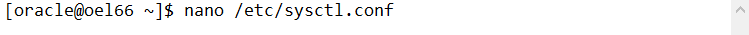
\includegraphics[width=12cm]{Imagenes/Oracle_Database/Paso_9.png}
\end{center}
\break
Una vez dentro del archivo, añadir al final de este la siguiente información:
\begin{center}
  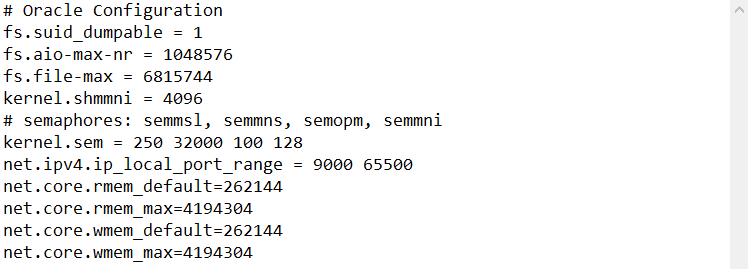
\includegraphics[width=12cm]{Imagenes/Oracle_Database/Paso_9_2.png}
\end{center}
\textbf {Paso 10.-} Se deberá ejecutar los cambios realizados, para lo cual ejecute la siguiente sentencia en el terminal.

\begin{center}
  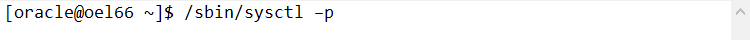
\includegraphics[width=12cm]{Imagenes/Oracle_Database/Paso_10.png}
\end{center}
Los resultados deberán ser similares a los siguientes
\begin{center}
  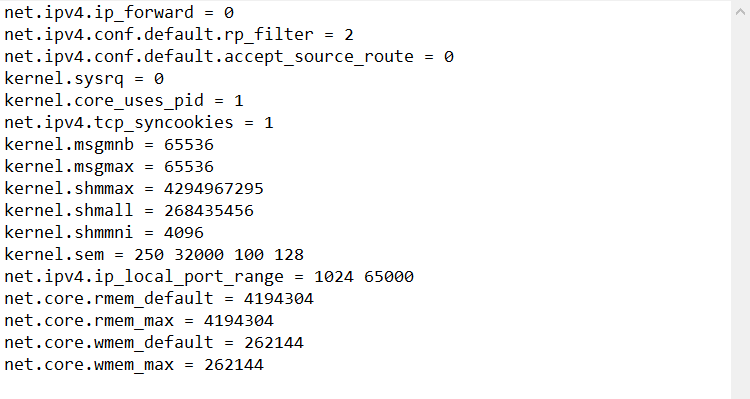
\includegraphics[width=12cm]{Imagenes/Oracle_Database/Paso_10_2.png}
\end{center}

\vspace{12pt}\\

\textbf {Paso11.-} Seguidamente se deberá realizar cambios a los límites de seguridad del sistema para el usuario oracle, para lo cual se debe editar el archivo /etc/security/limits.conf y adicionar las líneas siguientes al final del archivo.

\begin{center}
  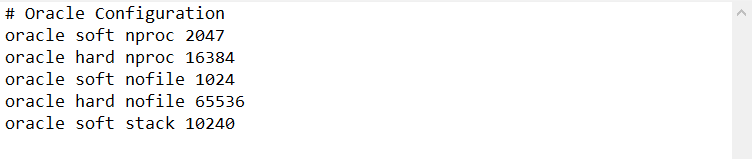
\includegraphics[width=12cm]{Imagenes/Oracle_Database/Paso_11.png}
\end{center}
\break

\textbf {Paso 12.-} Seguidamente se deberá configurar la interfaz de red y establecer una dirección IP estática para el servidor, para lo abrir el menú System (Sistema), el submenú Administration (Administración) y seleccionar la opción Networking (Red) y aparecerá la ventana configuración para establecer la Dirección IP. Seleccionar la interfaz de Red que se desea configurar y presionar el botón Edit (Editar).

\begin{center}
  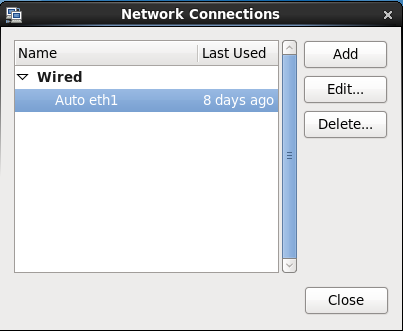
\includegraphics[width=8cm]{Imagenes/Oracle_Database/Paso_12.png}
\end{center}
\vspace{12pt}\\

\textbf {Paso 13.-} Dentro de la ventana de Configuración de la Interfaz de Red, seleccionar la opción de Statically set IP addresses (Establecer la dirección IP manualmente), luego introducir en los cuadros de texto la información necesaria, teniendo en cuenta las consideraciones iniciales:

\begin{center}
  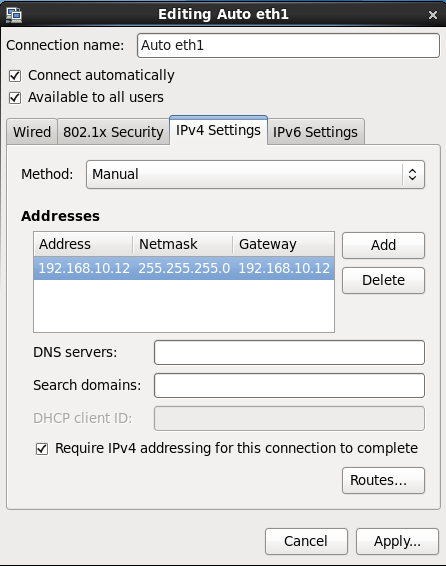
\includegraphics[width=9cm]{Imagenes/Oracle_Database/Paso_13.png}
\end{center}
\break

\textbf {Paso 14.-} Es necesario confirmar que se ha aplicado correctamente la configuración de red, para esto en la ventana de Terminal abierta. Escribir el siguiente comando:

\begin{center}
  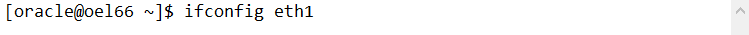
\includegraphics[width=12cm]{Imagenes/Oracle_Database/Paso_14.png}
\end{center}
Esto deberá retornar un resultado similar al siguiente:
\begin{center}
  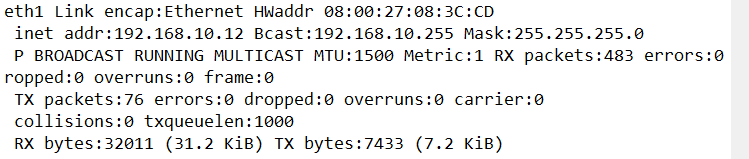
\includegraphics[width=12cm]{Imagenes/Oracle_Database/Paso_14_2.png}
\end{center}
\vspace{12pt}\\

\textbf {Paso 15.-} Luego de establecer satisfactoriamente la dirección IP de la interfaz de red, se debe configurar el nombre del servidor, para lo cual es necesario editar el archivo /etc/hosts (tener en consideración las consideraciones iniciales para establecer el nombre). Se deberá agregar la siguiente línea.

\begin{center}
  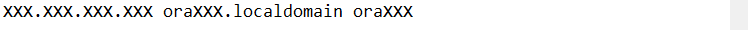
\includegraphics[width=12cm]{Imagenes/Oracle_Database/Paso_15.png}
\end{center}
\vspace{12pt}\\

\textbf {Paso 16.-} A fin de terminar la configuración del sistema con el usuario “root”, es necesario expulsar el DVD de instalación y reiniciar el sistema, para lo cual ejecutar los siguientes comandos:

\begin{center}
  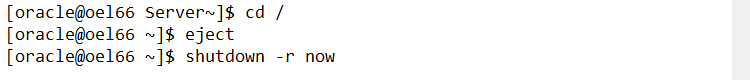
\includegraphics[width=12cm]{Imagenes/Oracle_Database/Paso_16.png}
\end{center}
\vspace{12pt}\\

\textbf {Paso 17.-} Después de reiniciar el sistema, iniciar sesión con el usuario “oracle“ (previamente creado).
\vspace{12pt}\\

\textbf {Paso 18.-} Una vez iniciada la sesión con el usuario “oracle”, abrir una ventana de Terminal y editar el archivo .bash_profile. Adicionar las siguientes líneas al final de este archivo:

\begin{center}
  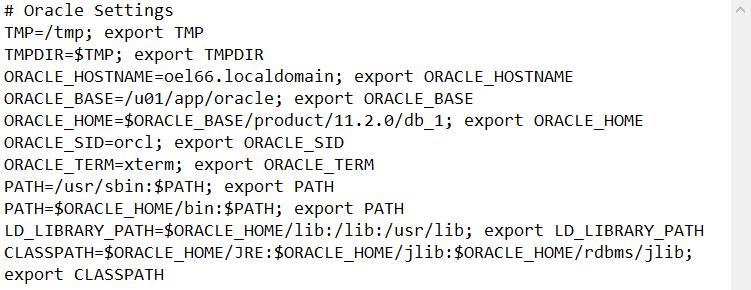
\includegraphics[width=12cm]{Imagenes/Oracle_Database/Paso_18.png}
\end{center}
\break

\textbf {Paso 19.-} Con la finalidad de que la configuración aplicada en el paso previo tenga efecto, es necesario reiniciar el sistema, para lo cual abrir el menú System (Sistema) ubicado en el panel superior, y presionar la opción Log Out (Salir de la sesión). Finalmente presionar el botòn Restart (Reiniciar).

\begin{center}
  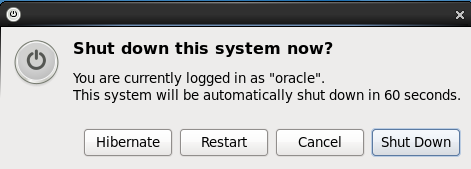
\includegraphics[width=11cm]{Imagenes/Oracle_Database/Paso_19.png}
\end{center}
\vspace{12pt}\\

\textbf {Paso 20.-} - Nuevamente en la ventana de inicio de sesión de Oracle Linux Server, iniciar sesión con el usuario “oracle”.
\vspace{12pt}\\

\textbf {Paso 21.-} Seguidamente montar en la unidad de CD/DVD el DVD con el archivo de instalación de Oracle Database Server o montar el archivo de tipo imagen (ISO) que contiene el archivo de instalación de Oracle Database Server.
\vspace{12pt}\\

\textbf {Paso 22.-} Ahora es necesario copiar los archivos de instalación de Oracle Database Server y luego descomprimirlo, para esto abrir una ventana de Terminal y ejecutar los siguientes comandos.

\begin{center}
  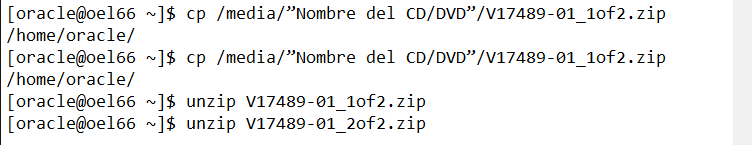
\includegraphics[width=12cm]{Imagenes/Oracle_Database/Paso_22.png}
\end{center}
\vspace{12pt}\\

\textbf {Paso 23.-} Una vez descompreso el archivo de instalación se creará una carpeta “/home/oracle/database”, a la cual se deberá acceder desde la ventana del Terminal y ejecutar el archivo de instalación, para lo cual ejecutar los siguientes comandos en el Terminal:

\begin{center}
  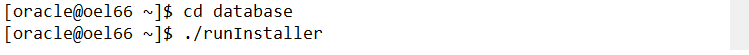
\includegraphics[width=12cm]{Imagenes/Oracle_Database/Paso_23.png}
\end{center}
\break

\textbf {Paso 24.-} A continuación se iniciará el programa de instalación de Oracle Database. En el paso 1 de 9 ingresar una dirección de correo electrónico (Email) válida y retirar el check sobre la opción Deseo recibir actualizaciones de seguridad vía Mi Soporte Oracle (I wish to receive security update vía My Oracle Support) y presionar el botón Next (Siguiente).

\begin{center}
  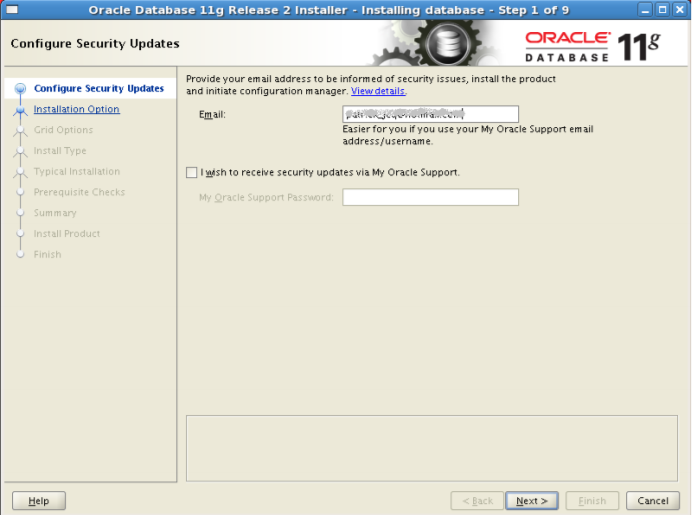
\includegraphics[width=12cm]{Imagenes/Oracle_Database/Paso_24.png}
\end{center}
\vspace{12pt}\\

\textbf {Paso 25.-} Si es que no se tuviese conexión a Internet, se visualizará el siguiente cuadro de dialogo de Fallo en la Conexión (Connection Failed), hacer click en la opción I want to remain uninformed of critical security issues in my configuration (Quiero permanecer desinformado de incidencia de seguridad críticas en mi configuración).

\begin{center}
  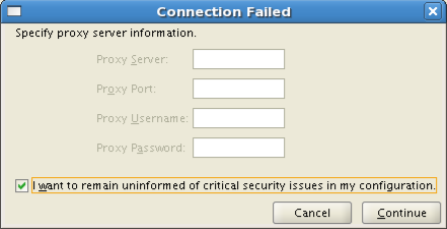
\includegraphics[width=11cm]{Imagenes/Oracle_Database/Paso_25.png}
\end{center}
\break

\textbf {Paso 26.-} En el paso 2 de 9, se deberá establecer las opciones de instalación, seleccionar la opción Crear y Configurar una base de datos (Create and configure a database) y presionar el botón Next (Siguiente).

\begin{center}
  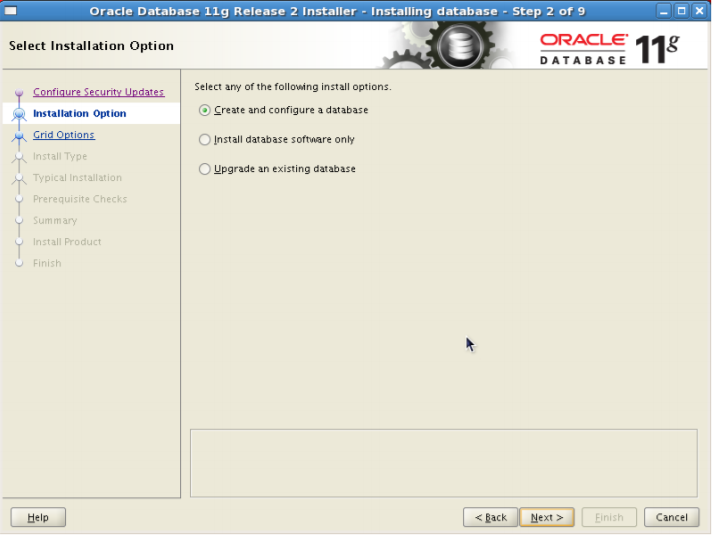
\includegraphics[width=11cm]{Imagenes/Oracle_Database/Paso_26.png}
\end{center}
\vspace{12pt}\\

\textbf {Paso 27.-} Seguidamente en el paso 3 de 8, Clase de Sistema, seleccionar la opción Clase Servidor (Server Class), luego presionar el botón Next (Siguiente).

\begin{center}
  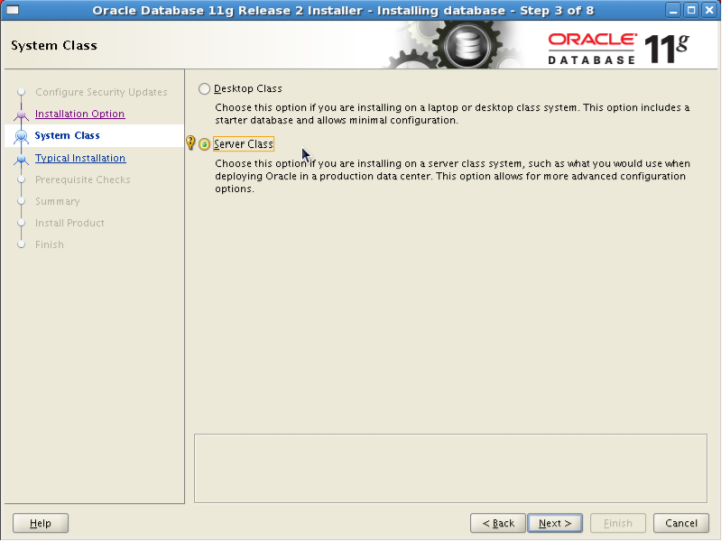
\includegraphics[width=11cm]{Imagenes/Oracle_Database/Paso_27.png}
\end{center}
\break

\textbf {Paso 28.-} En el paso de 4 de 10, Opciones de Grilla, Selección de Nodo, seleccionar la opción Instalación de base de
datos en instancia única (Single instance database installation), seguidamente presionar el botón Next
(Siguiente).

\begin{center}
  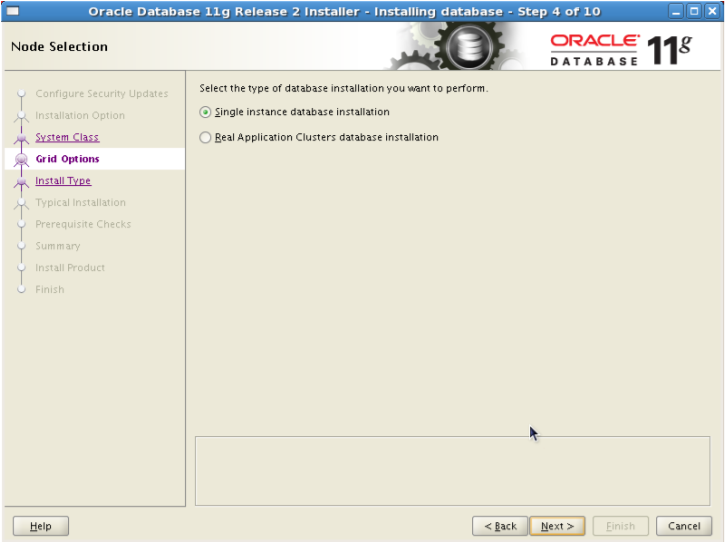
\includegraphics[width=11cm]{Imagenes/Oracle_Database/Paso_28.png}
\end{center}
\vspace{12pt}\\

\textbf {Paso 29.-} - En paso 5 de 10, Tipo de Instalación, seleccionar Instalación Típica (Typical install) y luego presionar el botón Next (Siguiente).

\begin{center}
  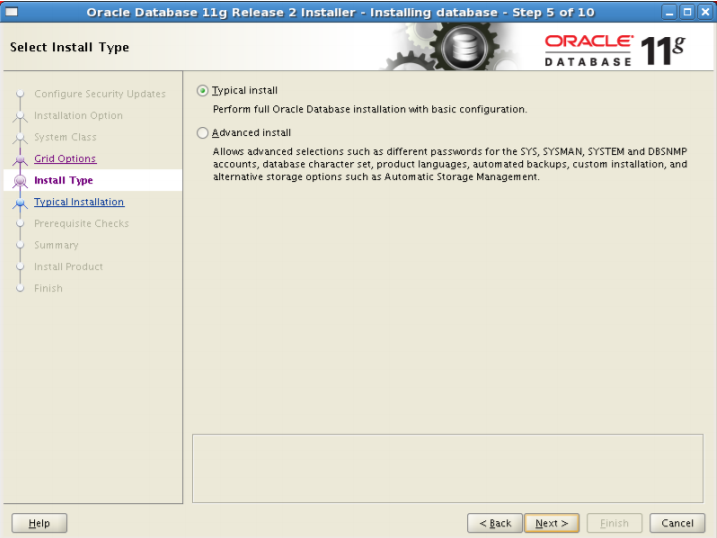
\includegraphics[width=11cm]{Imagenes/Oracle_Database/Paso_29.png}
\end{center}
\break

\textbf {Paso 30.-} Seguidamente en el paso 6 de 10, Configuración de la Instalación Típica, dejar los valores por defecto y establecer la contraseña para los usuarios administrativos (SYS, SYSTEM, SYSMAN y DBSNMP), para cual
debe introducir la palabra “oracle” en los cuadros de texto Administrative password (Contraseña de administración) y Confirm Password (Confirmar Contraseña). Una vez terminado esto presionar el botón Next (Siguiente).

\begin{center}
  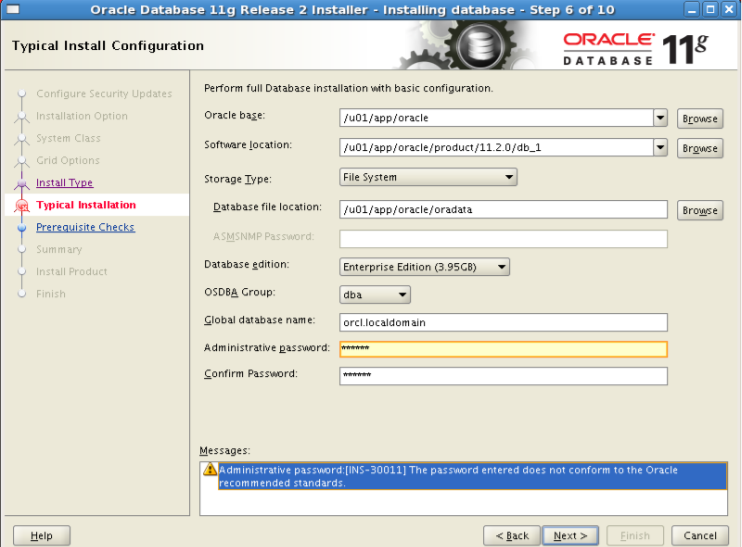
\includegraphics[width=11cm]{Imagenes/Oracle_Database/Paso_30.png}
\end{center}
\vspace{12pt}\\

\textbf {Paso 31.-} Debido a que la contraseña no cumple con los estándares recomendados por Oracle, se visualizará un cuadro de dialogo que solicitará la confirmación si se desea mantener la contraseña introducida, debido a que este es un laboratorio de pruebas la contraseña es suficiente, pero en un ambiente de producción se recomienda utilizar
una contraseña más segura. Presionar el botón Yes (Si) en el cuadro de dialogo.


\begin{center}
  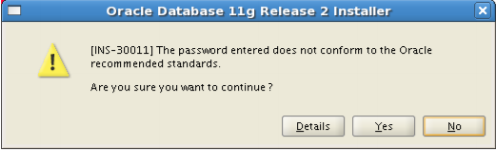
\includegraphics[width=11cm]{Imagenes/Oracle_Database/Paso_31.png}
\end{center}
\break

\textbf {Paso 32.-} Ahora, en el paso 7 de 11, se deberá establecer la ruta o ubicación donde los productos serán instalados así como el grupo de usuarios que tiene acceso a realizar modificaciones sobre esta ruta o esta ubicación. Dejar los valores por defecto y presionar el botón Next (Siguiente)

\begin{center}
  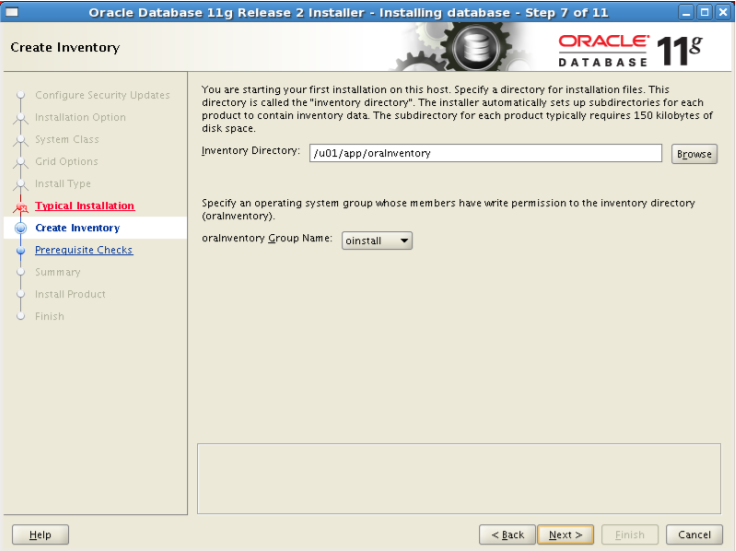
\includegraphics[width=11cm]{Imagenes/Oracle_Database/Paso_32.png}
\end{center}
\vspace{12pt}\\

\textbf {Paso 33.-} A continuación se el asistente de instalación de Oracle Database realizará la verificación de que todos los prerequisitos previos a la instalación hayan sido instalados y configurados correctamente. Si todas las
verificaciones han sido exitosas se continuará con el paso 9 de 11. Caso contrario si es que hubiese algún inconveniente con los requisitos, se mostrará el paso 8 de 11, con los errores detectados, verificar el detalle y corregir el paso incorrectamente ejecutado.

\begin{center}
  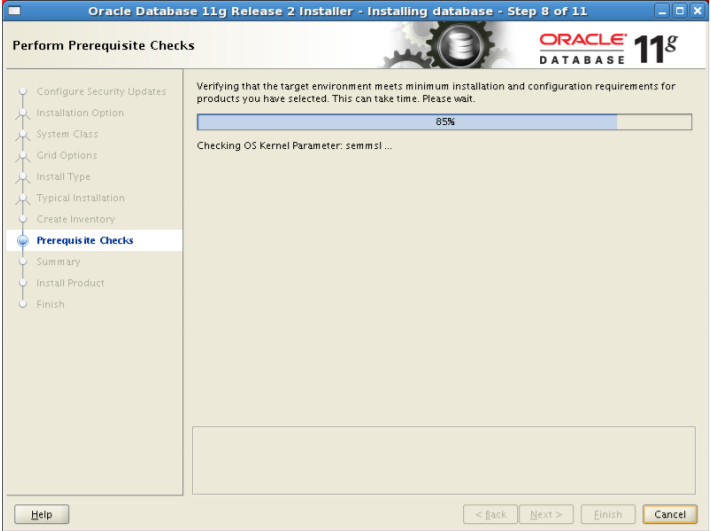
\includegraphics[width=11cm]{Imagenes/Oracle_Database/Paso_33.png}
\end{center}
\break

\textbf {Paso 34.-} Seguidamente, en el paso 9 de 11, aparecerá la pantalla de resumen de configuración previa a la instalación, la cual detalla todos los aspectos seleccionados para la presente instalación, revisar cada línea y luego para iniciar con la instalación presionar el botón Finalizar (Finish).

\begin{center}
  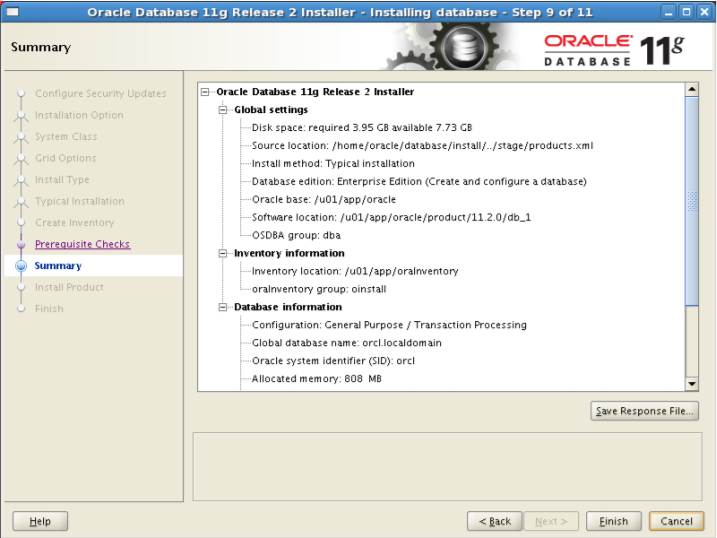
\includegraphics[width=11cm]{Imagenes/Oracle_Database/Paso_34.png}
\end{center}
\vspace{12pt}\\

\textbf {Paso 35.-} En el paso 10 de 11, se visualizará el proceso de instalación, se deberá esperar aproximadamente 15 minutos a que la instalación finalice y complete el 100 porciento.

\begin{center}
  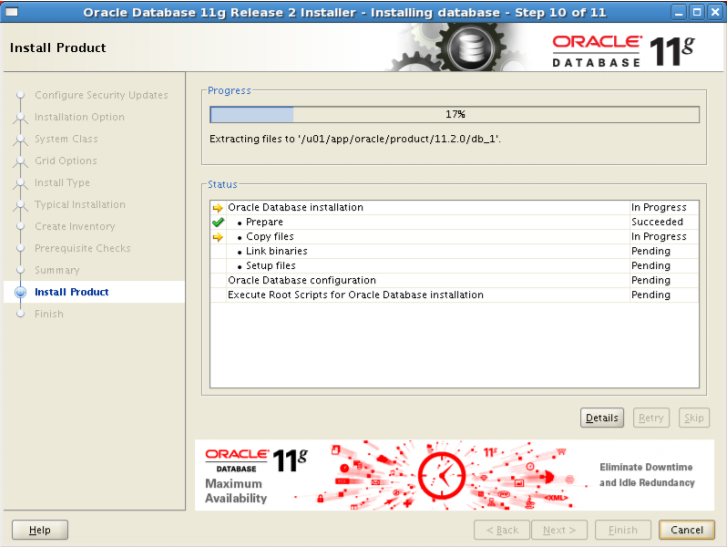
\includegraphics[width=11cm]{Imagenes/Oracle_Database/Paso_35.png}
\end{center}
\break

\textbf {Paso 36.-} Una vez completado el 100\% de la instalación, se iniciarán de manera automática el asistente de configuración  de Base de Datos de Oracle Database. Inmediatamente el Asistente de Configuración de Base de Datos, empezará con la creación de la instancia y luego procederá con la creación de la base de datos del sistema y la base de datos de ejemplo.

\begin{center}
  \includegraphics[width=11cm]{Imagenes/Oracle_Database/Paso_36.png}
\end{center}
\vspace{12pt}\\

\textbf {Paso 37.-} Una vez finalizada la personalización por parte del Asistente de Configuración de Base de Datos, el instalador de Oracle Database mostrará una pantalla resumen, en donde se indicará la instancia creada y la forma para ingresar a esta, mediante interfaz Web, tomar nota de estos datos y finalmente presionar el botón OK (Aceptar).

\begin{center}
  \includegraphics[width=10cm]{Imagenes/Oracle_Database/Paso_37.png}
\end{center}
\break

\textbf {Paso 38.-} A continuación se visualizará una pantalla que solicitará la ejecución de dos scripts que contienen comandos de configuración para el sistema.

\begin{center}
  \includegraphics[width=11cm]{Imagenes/Oracle_Database/Paso_38.png}
\end{center}
Para lo cual será necesario abrir una ventana de Terminal e iniciar sesión como usuario root, ejecutar los
comandos y cerrar sesión. Escribir los siguientes comandos en la ventana de Terminal y luego volver a la
ventana de ejecución de Comandos del instalador de Oracle Database y presionar el botón OK (Aceptar).
\begin{center}
  \includegraphics[width=11cm]{Imagenes/Oracle_Database/Paso_38_2.png}
\end{center}
\vspace{12pt}\\

\textbf {Paso 39.-} La siguiente pantalla mostrará la finalización del proceso de instalación. Tomar nota de dirección electrónica (URL) para hacer uso de la herramienta Enterprise Manager Database Control. Finalmente presionar el botón Exit (Salir).

\begin{center}
  \includegraphics[width=10cm]{Imagenes/Oracle_Database/Paso_39.png}
\end{center}
\break

\textbf {Paso 40.-} Como último paso y con la finalidad de verificar de que la instalación ha sido exitosa, iniciar un navegador de Internet (Mozilla u otro similar), e introducir la dirección electrónica de la cual se tomó nota en el paso anterior. Si todo es correcto aparecerá la interfaz de inicio de sesión de la herramienta Enterprise Manager (Administrador Empresarial) de Oracle.

\begin{center}
  \includegraphics[width=11cm]{Imagenes/Oracle_Database/Paso_40.png}
\end{center}
Una vez nos hayamos identificado correctamente, accederemos al Control de Base de datos.
\begin{center}
  \includegraphics[width=11cm]{Imagenes/Oracle_Database/Paso_40_2.png}
\end{center}
\vspace{12pt}\\

\end{enumerate}

    \section{CONSLUSIONES}
\begin{enumerate}
\vspace{12pt}

• Oracle es uno de los motores de base de datos relacional más utilizado a nivel mundial.\\
• Puede ejecutarse en todas las plataformas de hardware, desde una laptop, una PC, hasta en un supercomputador.\\
• Oracle soporta todas las funciones que se esperan de un servidor: un lenguaje de diseño de bases de datos muy completo (PL/SQL) que permite implementar diseños "activos", con triggers y procedimientos almacenados, con una integridad referencial declarativa bastante potente.\\
• Permite el uso de particiones para la mejora de la eficiencia, de replicación e incluso ciertas versiones admiten la administración de bases de datos distribuidas.\\
• En cuanto a seguridad, Oracle brinda al usuario un set de funcionalidades para obtener un ambiente muy seguro.\\

\end{enumerate}

    \section{BIBLIOGRAFIA}
\begin{enumerate}
\vspace{12pt}\\
\begin{flushleft}

Alexandra Del Valle Brito Gómez. (2019). Oracle. Noviembre 11, 2018, de Monografias Sitio web: https://www.monografias.com/trabajos25/oracle/oracle.shtml#in
\vspace{12pt}\\
Marvin Zumbado. (2012). Motor de base de datos Oracle. Noviembre 4, 2018, de SlideShare Sitio web: https://es.slideshare.net/moRado2/oracle-14874943
\vspace{12pt}\\
Equipo HP. (2018). Cómo activar y usar el cliente Hyper-V. Noviembre 4, 2018, de HP Sitio web: https://support.hp.com/pe-es/document/c04239922
\vspace{12pt}\\
Wikipedia. (2015). Oracle Database. Noviembre 12, 2018, de Wikipedia Sitio web: https://es.wikipedia.org/wiki/Oracle_Database

\end{flushleft}
\end{enumerate}

\end{document}
